\part{关于\LaTeX 的那些你想知道却从不敢问的问题}

\chapter{基本原则}
\begin{epigraphe}{《圣经·利未记》15:2}
    人若身患漏症,\\他因这漏症就不洁净了。
\end{epigraphe}

本章介绍\LaTeX 的基本原理。你将会看到关于\LaTeX 安装的简介、使用\LaTeX 的基本“流程”(session)介绍、文章格式的结构、使用变音符号的注意事项,认识几个工具,以及了解面对编译错误消息时的态度。

\section{安装}

你想安装\LaTeX 吗?你将要安装的是\LaTeX 的其中一个\textit{发行版},具体的版本取决于你的操作系统\jz{
    如果你不知道操作系统是什么东西,那么你使用的是macOS;如果你不知道你的计算机用的\textit{具体是哪个}操作系统,那么你在用Windows;否则,你在用UNIX……
}。发行版中带有可以自动安装和配置\LaTeX 、\TeX 和其他相关内容的程序。

\begin{description}
\item[对于UNIX]我们可以找到称为te\TeX 的发行版,虽然它的开发早在2006年就停止了。今天,我们一般安装\TeX Live(\wz{http://www.tug.org/texlive})。

\item[对于macOS]建议安装的发行版是Mac\TeX(\wz{http://www.tug.org/mactex})。

\item[对于Windows]最简单的方式无疑是选择pro\TeX t(\wz{http://www.tug.org/protext})。它会安装称为MiK\TeX 的发行版(\wz{http://www.miktex.org})和几个开发工具,其中包含一个查看PostScript文件的程序(\textsf{gsview})。

\end{description}

偶尔,需要在为发行版中搭配一款文字编辑器(如果其中没有包含),因为你很快就能看到,使用\LaTeX 就是在文件中输入文字和命令。

\begin{itemize}
    \item UNIX中,推荐使用\textsf{emacs}或\textsf{vi},即使前者明显比后者更高级,但二者用户之间无结果的恶意争吵仍在继续。
    \item \textsf{kile}和\textsf{texmaker}是已集成的开发环境。依靠它们,初学的用户在入门时会觉得更轻松。它们的特点是将编辑、编译和可视化集成在一个界面。这两个环境也使通过菜单、对话框或其他标签来探索\LaTeX 指令称为可能(如图\ref{fig:1.1}a所示)。
    \item Windows中的对应产品是\textsf{\TeX nicCenter}(如图\ref{fig:1.1}b所示)。
    \item macOS中的对应产品是\textsf{\TeX shop}和\textsf{i\TeX max}。
\end{itemize}

\begin{figure}%[H]
    %TODO 图
    \centering
    \includegraphics[width = 0.8\linewidth]{img/kile.eps}\\
    (a) Kile\\
    \includegraphics[width = 0.8\linewidth]{img/texniccenter.eps}\\
    (b) \TeX nicCenter
    \caption{集成的两个开发环境:Linux中的Kile和Windows中的\TeX nicCenter。它们将编辑、编译和可视化集成在一个界面中}
    \label{fig:1.1}
\end{figure}

你很快就会学到,用\LaTeX 制作文档是一个翻译(也称作\textit{编译})的过程——将编辑者创建的源文件转换为用于显示或印刷的格式\jz{本章会略微多介绍一些这个格式。}。因此,发行版中内置了或多或少的著名工具,可以将编译后的不同格式的文件显示出来。

\begin{description}

\item[对于PDF格式]除了著名的\textsf{acrobat reader},UNIX中还有一些可以显示PDF文件,如\textsf{xpdf}、\textsf{evince}等。

\item[对于DVI格式]UNIX中的\textsf{xdvi}、\textsf{kdvi}和Windows中的\textsf{yap}都是可以显示这种\LaTeX 编译文件的程序。

\item[对于PostScript格式]\textsf{ghostscript}套件(在各平台下的名称可能有差异)可以显示PostScript文件。

\end{description}

\begin{exclamation}
    需要注意,为了使你选用的发行版包含\LaTeX 的“法文”模式,以确保能够正确处理断字(césure;英:hyphenation),我们需要在编译文档是需要更改其“日志”(见1.6节)%带有引用
    以使法文模式加载:

    \begin{dmd}
    LaTeX2e <2005/12/01>\\
    Babel <v3.8h> and hyphenation patterns for english, [...] dumylang, \fbox{french}, loaded.
    \end{dmd}
\end{exclamation}

\section{“生产”周期}

即使\LaTeX 并不是通常意义上说的编译型语言,但我们仍然可以将制作一个\LaTeX 文档的周期与使用一款经典的编程语言开发软件的\textit{编辑—编译—执行}周期进行类比。

\subsection{编辑}

一个\LaTeX \textit{源}文件是一个文本文件\jz{即文件仅由组成其中符号的代码构成。}。因此,对\LaTeX 文件的操作并不依赖于某个特定的软件,只需要一个经典的文本编辑器即可。因此,若要操作\LaTeX 文档,指令

\dmh{emacs \codereplace{文件名}.tex \&} %TODO <>

或

\dmh{vi \codereplace{文件名}.tex}

足以让你进入\LaTeX 文档这个充满野性和未知的世界。在Windows中,根据自己的喜好,我们可以选用一款文字编辑器。注意,对于\LaTeX 源文件,推荐使用\dm{.tex}扩展名名。

\subsection{编译}

我们用如下指令开始编译:

\dmh{pdflatex \codereplace{文件名}.tex}

早晚有一天,你会看到编译会产出错误。这将是1.6节会处理的问题。总之,解决了编译问题后,我们会得到一个带有\dm{.pdf}扩展名的文件,它代表\textit{便携文档格式(英:portable document format)},这是一种由Adobe公司创造的著名格式。

\begin{ii}
    历史上,编译\LaTeX 源文件会生成\dm{dvi}文件,代表\textit{设备无关(英:device independant)}。此类文件独不受输出环境(如屏幕、打印机等)的影响。这是一种包含了“图像”的\LaTeX 便携二进制文件,可以用于各种操作系统。随后,出现了一批用途各异的程序:
    \begin{itemize}
        \item 用于显示文档,即\dm{.dvi}\rightarrow 点阵屏幕;
        \item 用于打印,即\dm{.dvi}\rightarrow 打印机语言;
        \item 用于转换格式,即\dm{.dvi}\rightarrow PostScript文件。
    \end{itemize}
\end{ii}

图\ref{fig:1.2}表明了UNIX生成最终文件过程中参与流程的多种程序。

\begin{ii}
    除了使用pdflatex外,也可以使用其他“编译器”来生成PDF文件。例如,xelatex和lualatex可以能正确地处理以UTF-8编码的文件,是常用的替代选项。
\end{ii}

\begin{figure}[H]
    %TODO 图
    \centering
    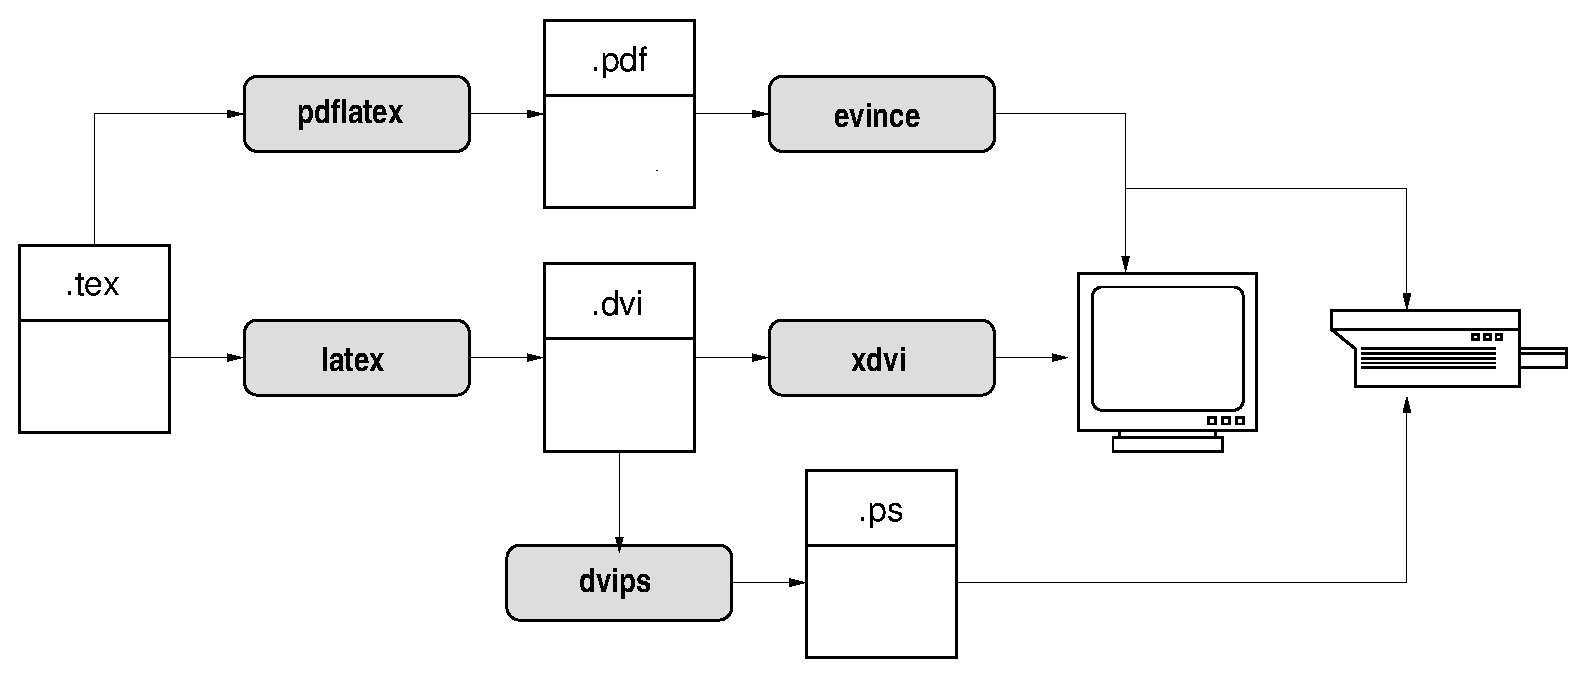
\includegraphics[width = 0.8\linewidth]{img/cycle.eps}
    \caption{UNIX中参与生成过程的工具}
    \label{fig:1.2}
\end{figure}

\subsection{显示}%visualisation有时翻译成可视化,有时翻译成显示,这个可以后期再统一一下。

在编译后,可以简单地使用\textsf{evince}程序来完成显示步骤。输入以下指令:

\dmh{evince \codereplace{文件名}.pdf \&}

这是一个\textsf{linux}下运行的十分直观的程序,能够给出一个方便阅读的文件预览。

\begin{exclamation}
    注意,不必在每次编译后都重新运行evince,它显示的内容会自动刷新。
\end{exclamation}

\subsection{打印}

对于\dm{pdf}格式,如何打印它这一问题就丢给了你的操作系统。关于这一点,没有特殊的注意事项。你有了一个文件,可以自由地处置它,无论是直接打印,还是根据你所处的环境来发挥才艺。

\begin{ii}
    从\dm{dvi}到\dm{ps}格式的转换需要调用dvips程序:

    \dmh{dvips \codereplace{文件名}.dvi}

    这可以生成一个PostScrpt格式的文件。这个格式也由Adobe创造,是一种打印机语言,可以看作\dm{pdf}的祖先。目前的打印机出厂即可识别这种打印机语言。我们可以说,文件发送到打印机时,十有八九传送的是PostScrpt格式的参数。对于PostScript格式的文件,有大量可以显示、修改这种文件的工具。
\end{ii}

\section{源文件的结构}

本节将介绍一种文档类型。实际上,所有\LaTeX 文档都具有相同的结构,形式如下:

\begin{dmd}
\backslash documentclass[\codereplace{类选项$_1$},\codereplace{类选项$_2$},...]\{\codereplace{类}\}\\
\backslash usepackage[\codereplace{包选项$_1$},\codereplace{包选项$_2$},...]\{\codereplace{包}\}\\
...\\
\codereplace{文前部分}\\
...\\
\backslash begin\{document\}\\
...\\
\codereplace{文本}\\
...\\
\backslash end\{document\}
\end{dmd}

如此一来,所有的\LaTeX 文档都可以按以下方式拆解。

\begin{itemize}
    \item 说明文档的\codereplace{类};
    \item 文前部分,包含以下内容:
        \begin{itemize}
            \item 使用特定的\codereplace{包};
            \item 多样的初始化和声明;
        \end{itemize}
    \item 文档主体,即我们将要亲手输入的全部内容,出现在\dm{\backslash begin\{document\}}和\dm{\backslash end\{document\}}之间。
\end{itemize}

以下介绍各部分的细节。

\subsection{文档的类}

所谓类,就是提供给\LaTeX 的一个指示,可以帮助\LaTeX 决定如何为文档的特定部分排版。根据具体使用的类不同,允许使用与否的指令可能不同(如\dm{\backslash chapter}在\dm{book}类中允许使用,在\dm{article}类中不允许使用)。另一方面,根据所选择的类,给出的命令会具有特定的含义(标题、材料表……)。在入门时\jz{
    实际上,我们可以在\dm{\backslash documentclass}前添加更多神奇的“咒语”……
},所有的\LaTeX 文档都必须以的指令开始——\dm{\backslash documentclass}接由花括号括住的类,包含以下几种:

\begin{itemize}
    \item \dm{article},用于文章;
    \item \dm{proc},用于电气与电子工程师协会(英:Institute of Electrical and Electronics Engineers,IEEE)会刊(英:proceeding)风格的文章;
    \item \dm{report},用于几十页篇幅的报告;
    \item \dm{book},用于图书或论文;
    \item \dm{letter},用于信件;
    \item \dm{slides},用于演示文档。
\end{itemize}

我们当然也可以为文档定义自己的类。类的配置项用方括号括住,可以是以下内容之一:

\begin{itemize}
    \item \dm{11pt, 12pt},用于全局地更改文字字号;
    \item \dm{twoside},用于生成适合双面打印的文档;
    \item \dm{draft},用于以草稿模式生成文档。
\end{itemize}

例如,输入:

\begin{dmd}
\verb|\documentclass{article}|
\end{dmd}

以上命令可以将全部配置项配置为默认值(字号为10 pt,单列,单面……)。

\begin{dmd}
    \backslash documentclass[12pt]\{article\}
\end{dmd}

以上命令将字号设置为12 pt(默认为10 pt)。再如:

\begin{dmd}
    \backslash documentclass[twoside, draft]\{report\}
\end{dmd}

以上命令可以以草稿模式生成适合双面打印的报告。

\subsection{文前部分}

文前部分是指位于子句\dm{\backslash documentclass}和子句\dm{\backslash begin\{documennt\}}间的区域。在这个区域中,我们可以明确想要包含的扩展(请看下一小节)%TODO
、初始化全局参数(如页边距等)、定义风格(如标题样式、序号等)、定义特殊的宏,等等。

\subsection{添加扩展}

\LaTeX 命令\dm{\backslash usepackage}可以与C语言的指令\dm{\#include}类比。这一命令允许添加\LaTeX 中满足宏或环境形式的功能\jz{
    相关内容将在下一章讲解。%TODO
}。目前,只需记住,我们可以在一行之内包含多个包:

\begin{dmd}
    \backslash usepackage\{\codereplace{包$_1$},\codereplace{包$_2$},\codereplace{包$_3$},...\}
\end{dmd}

如果\codereplace{包$_1$}、\codereplace{包$_2$}、\codereplace{包$_3$}拥有共同的配置项\codereplace{opt1},我们可以输入:

\begin{dmd}
    \backslash usepackage[\codereplace{opt1}]\{\codereplace{包$_1$},\codereplace{包$_2$},\codereplace{包$_3$}\}
\end{dmd}

相反,如果\codereplace{opt1}只涉及\codereplace{包$_2$},那么我们只能像这样写成两行:

\begin{dmd}
    \backslash usepackage\{\codereplace{包$_1$},\codereplace{包$_3$}\}\\
    \backslash usepackage[\codereplace{opt1}]\{\codereplace{包$_2$}\}
\end{dmd}

下面是两个例子:

\begin{dmd}
    \% 包graphicx带有配置项draft和xdvi\\
    \backslash usepackage[xdvi, draft]\{graphicx\}\\
    \% 包array和包subfig\\
    \backslash usepackage\{array, subfig\}
\end{dmd}

\begin{exclamation}
    根据定义,所有(类、包、命令的)的配置项参数都是\textit{可选的}。因此我们可以这样记:\LaTeX 中所有由方括号括住的参数\dm{[...]}都是非强制的。
\end{exclamation}

\section{开始!}

在本节,我们将尝试从一个只含几个排版命令的文档开始,介绍\LaTeX 的基本原理。

\begin{codelist}[1.1]{
    从你手中掉落的工具总是掉到最难够到的地方,或脆弱的物品上。\\
    这是\emph{墨菲}定律(loi de Murphy)的一个体现。
}
\begin{verbatim}
\documentclass{article}
\begin{document}
从你手中掉落的工具
总是掉到最难够到的地方,
或脆弱的物品上。

这是\emph{墨菲}定律(loi de      Murphy)的
一个体现。
\end{document}\end{verbatim}
\end{codelist}

这个示例体现了\LaTeX 中的几个重要的原理,具体如下。

\begin{description}


\item[空行代表跳转至下一段] \LaTeX 中的空行代表一段文字的结尾,因此在以上实例中,第一段从“\dm{从你}”开始,直到“\dm{物品上。}”结束。指令\dm{\backslash par}与空行等价,可以用来表示一段文字的起始。

\item[\LaTeX 会忽略换行]最终的文档中,换行并不由源文件中的换行决定。\LaTeX 会自动为各段文本\textit{打断、压缩、调节}文字,除非你有特殊的要求。

\item[\LaTeX 会忽略重复的空格]输入1个或18784个空格是等价的,比如源码中\dm{de}和\dm{Murphy}前插入的空格那样。此规则也适用于跳转段落:输入一行或多行空格是等价的。

\item[“\backslash ”是转义字符(caractère d’échappement;英:escape char)]“\backslash ”可以告诉\LaTeX 它后面的一系列字符是控制序列,也就是说,是最一般意义上的指令(或宏)。这里,它对“墨菲”一词生效,具体的效果由指令\dm{\backslash emph}控制。

\item[“\{”和“\}”]它们是\textit{组}的定界符,稍后会进一步解释它们。

\end{description}

\subsection{几个特殊字符}

就像符号“\backslash”的出现所暗示的那样,\LaTeX 中还有10个有特殊含义的符号,在此将其列出:

\begin{dmd}
    \verb+\ $ & % # ^ _ { } ~+
\end{dmd}

%todo 此前代码可以重新简化为verb

以下是一个使用部分特殊字符的案例:

\begin{codelist}[1.2]{
\textbf{是}下标:$x_{i+1}$,还是上标:$e^{i\pi}$;这是问题~1!
}
\begin{verbatim}
%毫无意义的段落
\textbf{是}下标:$x_{i+1}$,
还是上标:$e^{i\pi}$;
这是问题~1!%还是问题2?\end{verbatim}
\end{codelist}

目前,你需要知道:

\begin{itemize}
    \item \dm{\%}会使得\LaTeX 忽略当前行的剩余部分,因此,它是表示注释的符号(与C中的\dm{//}等价);
    \item \verb+~+代表不可拆分的空格\jz{
        见2.10节。
    },可以防止\LaTeX 在指定的位置断字。尽管有大量的情况需要插入这个符号来表示不可拆分(如所有形如“\verb+图~1+”的情况),然而,对于此类符号的使用,并没有系统化的规则。
    \item \dm{\$}用于标记公式的开始和结束。\LaTeX 遇到一个\dm{\$}符号时,它会切换到\celan{第3章}数学模式,直到遇到下一个\dm{\$}符号。
    \item \dm{\_}和\dm{\^{}}分别代表将文本转化为下标和上标。\textbf{注意},这两个符号只能在数学模式下使用。
    \item \dm{\{}和\dm{\}}分别表示组的开始和结束。本例中出现了两种组:一种出现在数学模式中,用于把将要放到下标或上标的“子公式”组合起来;另一种把将要设置成粗体的文字组合起来。
\end{itemize}

我们可以使用如下的指令来在让文档生成部分特殊字符:

\begin{dmd}
    \verb+\$ \& \% \# \{ \} \_+
\end{dmd}

这串指令可以输出“\$ \& \% \# \{ \} \_”。2.2.5小节%TODO
会解释如何使文档生成其余特殊字符(即\verb+\ ~ ^+)。

\subsection{调用指令}

你已经知道了,要想调用指令或宏,需要输入转义字符,并紧接着输入你想使用的宏名。%TODO 二对一
但是,\LaTeX 如何知道宏名的末尾在哪里呢?此处以用于生成\TeX 标识的\dm{\backslash TeX}为例来解释\yz{
    此例涉及对西文行文中空格的处理,不宜翻译。
}。

\begin{codelist}[1.3]{
    \TeX book is for \TeX hackers.

    \TeX\  has some powerful macros.

    \LaTeX{} is a document preparation system
}
\begin{verbatim}
\TeX book is for \TeX hackers.

\TeX\  has some powerful macros.

\LaTeX{} is a document preparation system\end{verbatim}
\end{codelist}

\begin{exclamation}
    \verb*|\ |(其中\verb*| |代表空格)称作控制空格(espace de contrôle)。这个空格不会被\LaTeX 忽略。因此,指令“\verb*|et\ \ \ hop !|”会生成“et\ \ \ hop !”。实际上,以\dm{\backslash}\codereplace{函数}\dm{\{}\codereplace{参数}\dm{\}}的形式来调用宏是很好的习惯。因此,使用上例中的的第三种方式比第二种方式更佳。这种形式可以避免空格被忽略的情况发生\jz{
        所以他为什么要跟我们说这些?!
    }。因此,我们将使用\verb|the \teX{}book|来生成“the \TeX{}book”,使用“\verb*|\LaTeX{} is a ...|”来生成“\LaTeX{} is a ...”。
\end{exclamation}

\subsection{变音符号}

法国人往往对于使用\LaTeX 这件事忧心忡忡,因为法文中带有变音符号。别怕!你不必像表\ref{tab:1.1}\yz{
    该表与原书不完全相同。
}中展示的那样输入带有变音符号的字符。然而,你需要知道:无论是什么种类的字符,包括大写字母,我们都可以为其添加变音符号。

\begin{table}[H]
    \centering
    \begin{tabular}{|c|c|c|}
        \hline
        变音符号 & 源码 & 效果\\
        \hline
        尖音符 & \verb|\`z| & \`z \\
        钝音符 & \verb|\'z| & \'z \\
        长音符 & \verb|\^z| & \^z \\
        软音符 & \verb|\c{z}| & \c{z}\\
        分音符 & \verb|\"{z}| & \"{z}\\
        \hline
    \end{tabular}
    \caption{输入占7位(bit)的变音符号}
    \label{tab:1.1}
\end{table}

注意!虽然我们可以输入带有变音符号的字符,但不要忘记:这需要我们调用编码。目前,编码可能只针对地球上的某个地区。在法国,我们使用ISO 8859编码,配合拉丁文1区拓展。这套编码允许我们操纵美丽的变音符号。在详细阅读本书中专为使用法文书写文档的情况准备的章节\celan{第7章}之前,我们建议你在你源码的文前部分添加以下指令,以“攻克”法文文档的难关:

\begin{dmd}
    \begin{verbatim}
%源文件编码
\usepackage[latin1]{inputenc}
%TeX字体编码
\usepackage[T1]{fontenc}
%针对法文文档
\usepackage[francais]{babel}
    \end{verbatim}
\end{dmd}

\section{第一批工具}

以下几个宏和合字在文档中很常用,因此应当了解它们。首先,\LaTeX 会区分三种连接号:

\begin{itemize}
    \item \verb|-|,用于“Saint-Étienne”;
    \item \verb|--|,用于“page 12--24”;
    \item \verb|---|,在法文中用于插入语,如“une parenthèse --- comme cela”。
\end{itemize}

引号应以如下方式输入:

\begin{itemize}
    \item \verb|``|和\verb|''|可以输入英文中的引号\yz{
        此处与原书不同。原书前文输入变音符号时亦直接使用了单弯引号‘和’,但这两个符号作为命令参数时会导致编译错误,因此分别替换为反引号和直单引号。这可能是编译器的差异导致的。
    }——``English''。
    \item 如果键盘允许,对于法文,你可以输入«和»\jz{
        例如,在Linux系统下,分别按键盘的组合键\ovalbox{Alt Gr}+\ovalbox{Z}和\ovalbox{Alt Gr}+\ovalbox{X}(译注:适用于AZERTY键盘)。
    }。\textsf{babel}包的法文支持部分(参考第7章)%TODO
    允许我们通过\verb|\og|和\verb|fg|输入引号,由此,\verb|\og français\fg{}|这类命令是允许的—— «~français~»~。
\end{itemize}

以下是其余几个使用的命令:

\begin{itemize}
    \item \verb|\today|可以生成(编译时的)日期——2013年11月22日。
    \item \verb|\S|可以生成段落符号——\S。
    \item \verb|\ldots|可以在英文文档中生成省略号“\ldots”。但在法文文档中,应当输入三个点“...”(第7章会介绍更多有关法文排版的内容)。%TODO
\end{itemize}

最后要记得,英文中的双成分标点(ponctuation double;包括: ; ! ?)前不加空格,但法文相反,它们的前面需要加空格。另外,在法国这个可爱的国家,我们几乎都靠右行驶。

\section{第一组报错}

\begin{ii}
    接下来,我们会看看\LaTeX 编译你的文档时闹的“情绪”。当我们放出编译指令时,我们会直接在终端看到这些输出。为了能让\LaTeX 得到充分使用,我们鼓励你在自己的环境下找到属于你自己的检查\LaTeX “\textsf{日志}”的方法。这些日体可以为你指明错误信息,以及编译过程中出现的其他警告。
\end{ii}

\subsection{症状}

如果你与\LaTeX 打交道,那么早晚有一天,你会看到屏幕上显示出类似这样粗旷的信息:

\begin{dmd}
    \linenumbers
    \begin{verbatim}
This is TeX, Version 3.1415 (C version 6.1)
(erreur.tex
LaTeX2e <1995/12/01>
(/usr/local/lib/texmf/tex/cls/article.cls
Document Class: article 1995/11/30 v1.3p Standard LaTeX document class
(/usr/local/lib/texmf/tex/clo/size10.clo)) (erreur.aux)
! Undefined control sequence.
l.5 paragraphe de ce \empha
                           {document}
?\end{verbatim}
\end{dmd}

几乎可以肯定,你看不懂这团内容。它是使用\LaTeX 处理文件\dm{erreur.tex}后终端上显示的内容。以下是文件全文\yz{
    文件正文意为:\dm{我觉得,在这样短的\backslash empha\{文档\}的第一段就有一个错误}。
}:

\begin{dmd}
    \begin{verbatim}
\documentclass{article}

\begin{document}
Il me semble bien qu’il y ait une erreur dans le
premier paragraphe de ce \empha{document} somme
toute assez court.
\end{document}
    \end{verbatim}
\end{dmd}

\subsection{诊断}

我们可以以一种简单的方式来解释以上错误信息。

\begin{description}

\item[第1行]你使用的\TeX 版本为$\pi\pm 10^{-4}$。
\item[第2行]你想编译文件\dm{erreur.tex}。
\item[第3行]你使用了\LaTeXe ,版本日期为1995年12月。
\item[第4行~第5行]你使用了标准文档类\dm{article}。
\item[第6行]字号默认设置为10 pt。
\item[第7行]错误信息本身。
\item[第8行~第9行]\dm{erreur.tex}中造成错误的代码行和对应行号。
\item[第10行]\TeX 给出的短促且尤其让人焦虑的消息:\dm{?}。

\end{description}

第8行和第9行之间的“裂缝”精准地表明了\LaTeX 崩不住了的地方。以下消息:

\begin{dmd}
    ! Undefined control sequence.
\end{dmd}

向你说明了,\LaTeX 不认识你输入的指令。实际上,指令\verb|\empha|不存在。

\subsection*{治疗方案}

那么,当\LaTeX 给我们展示这个著名的“\dm{?}”时,我们应该怎么回答它呢?这里有3种最简短的方式,可以用来与\LaTeX 轻度交流。

\begin{itemize}
    \item 按回车键来忽略错误。
    \item 输入\dm{x}来退出编译。
    \item 输入\dm{r}让\LaTeX 继续编译,并忽略其他错误信息。
    \item 输入\dm{i}以插入一条更正信息并继续编译,但新插入的更正信息并不会出现在源文档中。
    \item 输入\dm{h}以获取更多关于该错误的信息。以下是本例中\TeX 提供给你的更多信息:\begin{verbatim}
Undefined control sequence :
  The control sequence at the end of the top line
  of your error message was never \def’ed. If you have
  misspelled it (e.g., ‘\hobx’), type ‘I’ and the
  correct spelling (e.g., ‘I\hbox’). Otherwise just
  continue, and I’ll forget about whatever was
  undefined.\end{verbatim}
\end{itemize}

\subsection{一些消息}

\TeX 和\LaTeX 会根据不同的情况给出大量错误消息,其中有一些在第一次面对时并不能读懂。然而,大多数经常出现的消息有以下类型:

\begin{itemize}
    \item \LaTeX 语法或保留字错误;
    \item 花括号没有成对出现;
    \item 在文本模式中出现了本应出现在数学模式中的内容;
    \item 数学模式没有关闭;
    \item 你忘记包含一个包;
    \item 编译过程无法结束;%TODO核实
    \item ……
\end{itemize}

\section{再说几句!}

现在,你知道了如何用\LaTeX 源码创建可打印的文件。同时,本章向你介绍了调用指令的原则。接下来,如果想要了解\LaTeX 语法中的不同功能,需要做的仅仅是去着手接下来的章节。%TODO